\scanpage{3}
We thus have an exact sequence
\diagram{\begin{tikzcd}[ampersand replacement=\&,column sep=large]
{(6)}\&1\arrow[r]\&\pi_1(X)\arrow[r]\arrow[d,equal]\&\mathcal E_X\arrow[r]\&\mathcal G_X\arrow[r]\arrow[d]\&1\\
\&\&\operatorname{Aut}(\widetilde X/X)\&\&\Gamma\&
\end{tikzcd}}
\deleted{The datum of a point}

Let us consider a point \unsure{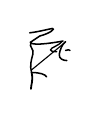
\begin{tikzpicture}[x=.008cm,y=-.008cm,baseline=(xibase.base),line cap=round,line join=round]
\node[inner sep=0pt] (xibase) at (1038,561) {\phantom{$x$}};
% The xi and adjacent X-like overwork are kept at their visible relative positions.
\draw[line width=.55pt] (1022,521)..controls(1037,519)and(1048,516)..(1058,514)
 ..controls(1064,514)and(1054,522)..(1038,526)--(1023,536)
 ..controls(1024,541)and(1048,539)..(1075,534);
\draw[line width=.55pt] (1024,537)..controls(1020,543)and(1030,547)..(1027,555)
 ..controls(1024,566)and(1022,573)..(1025,584)
 ..controls(1038,584)and(1047,587)..(1049,591);
\draw[line width=.65pt] (1025,584)..controls(1028,597)and(1024,603)..(1024,610);
\draw[line width=.5pt] (1073,535)..controls(1069,541)and(1056,544)..(1055,548)
 ..controls(1057,552)and(1063,550)..(1065,551);
\draw[line width=.55pt] (1079,535)..controls(1073,539)and(1070,549)..(1069,555)
 ..controls(1068,562)and(1075,565)..(1081,565);
\draw[line width=.4pt] (1026,579)--(1076,538);
\draw[line width=.55pt] (1079,549)..controls(1083,547)and(1085,548)..(1086,549);
\end{tikzpicture}}
\[
(7)\qquad\xi\in X(\overline{\mathbf Q})
\]
and let $\mathcal G_X(\xi)\subset\mathcal G_X$ be the subgroup
of $\mathcal G_X$ which fixes $\xi$. (NB. If 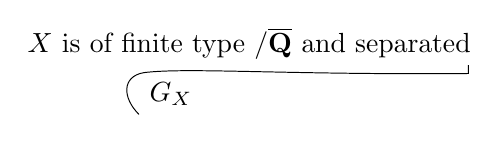
\begin{tikzpicture}[baseline=(gx.base)]
\node[anchor=base west,inner sep=0pt] (gx) at (1.55,0) {$G_X$};
\node[anchor=base west,inner sep=0pt] (nbinsert) at (0,.62)
 {\inserted{$X$ is of finite type $/\overline{\mathbf Q}$ and \unsure{separated}}};
% The under-running line bends down on the left to attach before G_X.
\draw[line width=.35pt] ([xshift=-1pt,yshift=-2pt]nbinsert.south east)
 -- ([xshift=-1pt,yshift=-5pt]nbinsert.south east)
 ..controls(3.30,.33)and(2.03,.43)..(1.48,.36)
 ..controls(1.20,.31)and(1.21,.04)..(1.42,-.17);
\end{tikzpicture} is
finite, $\mathcal G_X$ is profinite and $\mathcal G_X(\xi)$ is an
open subgroup\ldots). We then find,
if we choose for $\widetilde X$ the universal covering
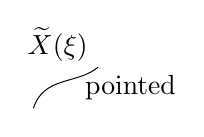
\begin{tikzpicture}[baseline=(pointed.base)]
\node[anchor=base west,inner sep=0pt] (pointed) at (.75,0) {pointed};
\node[anchor=base west,inner sep=0pt] at (.02,.50) {\inserted{$\widetilde X(\xi)$}};
\draw[line width=.35pt] (.92,.34)..controls(.66,.12)and(.23,.23)..(.10,-.18);
\end{tikzpicture} over $\xi$, a
partial splitting of (6)
\diagram{
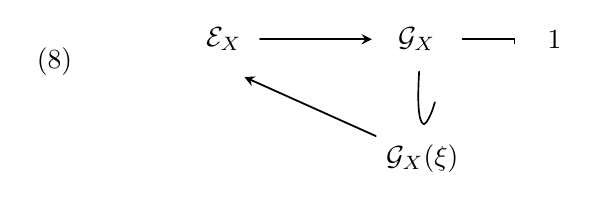
\begin{tikzpicture}[>=stealth,line cap=round,line join=round]
\node at (-2.15,-.28) {$(8)$};
\node[inner sep=0pt] (ex) at (0,0) {$\mathcal E_X$};
\node[inner sep=0pt] (gg) at (2.45,0) {$\mathcal G_X$};
\node[inner sep=0pt] at (4.20,0) {$1$};
\node[inner sep=0pt] (stab) at (2.52,-1.52) {$\mathcal G_X(\xi)$};
\draw[line width=.65pt,->] (.46,0)--(1.88,0);
% The right horizontal stroke ends in a short downward tick, not a two-wing head.
\draw[line width=.55pt] (3.03,0)--(3.69,0)--(3.69,-.055);
% Tall open U with the left arm longer than the right; no arrowhead is supplied.
\draw[line width=.6pt] (2.48,-.41)..controls(2.46,-.74)and(2.46,-1.05)..(2.54,-1.08)
 ..controls(2.59,-1.06)and(2.65,-.91)..(2.68,-.80);
\draw[line width=.65pt,->] (1.93,-1.23)--(.26,-.48);
\end{tikzpicture}
}
In the case where $\widetilde X$ is arbitrary, we
only find a homomorphism modulo composition
with inner automorphisms coming from
$\pi_1(X)$. \deleted{If $X$ is of finite type and}
\mspage{2}
